% 第3章第3节：热方程与扩散（扩散方程与模式衰减；弱演化与解算子；能量、正性与长期极限）。

\section{热方程与扩散}
\label{sec:pde-heat}

上一节的场不随时间变化。本节让场动起来：热量从热处流向冷处，温度场随时间被抹平。我们先从守恒关系推出方程，用可以直接验证的正弦模式看清“高频衰减更快”；再在函数空间中建立弱解与解算子，把热方程放进与上一章矩阵指数平行的框架；最后研究能量、总热量、正性和长期极限。

\subsection{扩散方程与模式衰减}
\label{sec:pde-heat-modes}

\paragraph{从守恒与通量得到热方程}
回到细棒。设棒的密度为$\rho$、比热为$c$，截面积取为$1$，温度为$u(x,t)$。区间$[a,b]$中的热量是$\int_a^b\rho cu\,\mathrm dx$。记$q(x,t)$为单位时间内向右穿过截面$x$的热量，$s(x,t)$为单位长度的热源功率。热量守恒说：$[a,b]$中热量的变化率，等于从左端流入的、减去从右端流出的，再加上内部产生的，
\[
  \frac{\mathrm d}{\mathrm dt}\int_a^b\rho cu\,\mathrm dx=q(a,t)-q(b,t)+\int_a^bs\,\mathrm dx .
\]
这是一个积分形式的平衡，还没有说明热流由什么决定。\term{Fourier定律}（Fourier's law）补上这一步：热流与温度梯度成正比、方向相反，$q=-k\,u_x$，$k>0$为导热系数。热总是从热处流向冷处。

设各量足够光滑，把$q(a)-q(b)=-\int_a^bq_x\,\mathrm dx$代入，得$\int_a^b(\rho cu_t-(ku_x)_x-s)\,\mathrm dx=0$。它对所有$a<b$成立，被积函数又连续，只能处处为零。系数为常数时，令$\kappa=k/(\rho c)$、$f=s/(\rho c)$，得到\term{热方程}（heat equation）
\begin{equation}
  u_t=\kappa u_{xx}+f .
  \label{eq:pde-heat-1d}
\end{equation}
$\kappa$称为\term{扩散系数}（diffusion coefficient）。在$d$维区域中，同样的推理把端点通量换成穿过任意小区域边界的通量，用散度定理得到$u_t=\nabla\cdot(\kappa\nabla u)+f$，常系数时即$u_t=\kappa\Delta u+f$。边界上的热交换就是第~\ref{sec:pde-boundary-solution-meaning}小节的三类边界条件。

式~\eqref{eq:pde-neighbor-average}给出了这个方程的直观读法：$\kappa u_{xx}\approx(2\kappa/h^2)\bigl(\text{邻居平均值}-u\bigr)$。每一点都以正比于“自己与邻居之差”的速率向邻居的平均值靠拢，比邻居高的地方降温，比邻居低的地方升温。下面取$\kappa=1$；一般的$\kappa$只需把时间换成$\kappa t$。

\paragraph{正弦模式的指数衰减}
在$(0,1)$上取两端为零的Dirichlet条件，无源。不急于解一般的初值，先猜一个形状不变、只按比例缩小的解$u(x,t)=a(t)\sin(k\pi x)$，$k$为正整数。它满足两端为零；代入方程，$a'(t)\sin(k\pi x)=-k^2\pi^2a(t)\sin(k\pi x)$，所以$a(t)=a(0)e^{-k^2\pi^2t}$。

于是每个正弦形状都是一个\term{特征模式}（eigenmode）：它在演化中保持形状，振幅按$e^{-\lambda_kt}$衰减，衰减率$\lambda_k=k^2\pi^2$随频率的平方增长。振幅减半所需的时间是$\ln2/\lambda_k$：$k=1$时约为$0.070$，$k=4$时约为$0.0044$，相差$16$倍。原因在式~\eqref{eq:pde-neighbor-average}中：$\sin(k\pi x)$的曲率$k^2\pi^2\sin(k\pi x)$随频率平方增大，振荡越快，每个峰与邻居的落差相对越大，被抹平得越快。

\paragraph{叠加与高频更快衰减}
方程是线性的，模式可以叠加。图~\ref{fig:pde-heat-modes}(a)的初值是$\sin(\pi x)+\tfrac12\sin(4\pi x)$：高频的小起伏在$t=0.015$时已几乎看不见，剩下的是缓慢下降的最低模式；图~\ref{fig:pde-heat-modes}(b)在对数坐标中画出各模式的振幅，它们是斜率为$-k^2\pi^2$的直线。

\begin{figure}[!htb]
  \centering
  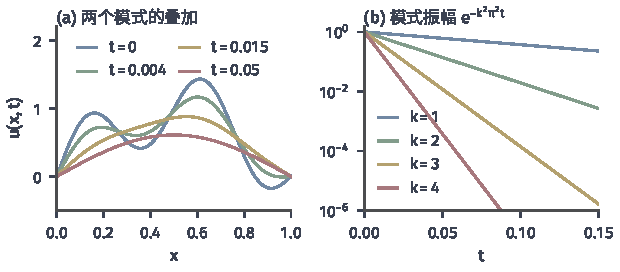
\includegraphics[width=105mm]{figures/03-optimization-evolution-and-signals/02-processes-and-trajectory-evolution/matplotlib/pde-heat-modes/figure.pdf}
  \caption{热方程$u_t=u_{xx}$在两端为零时的模式衰减。(a)~初值$\sin(\pi x)+\tfrac12\sin(4\pi x)$的解$e^{-\pi^2t}\sin(\pi x)+\tfrac12e^{-16\pi^2t}\sin(4\pi x)$在四个时刻的形状，高频起伏先消失。(b)~第$k$个模式的振幅$e^{-k^2\pi^2t}$，纵轴为对数刻度，斜率$-k^2\pi^2$。}
  \label{fig:pde-heat-modes}
\end{figure}

一般的初值能否写成这些模式的叠加？需要两件事：模式两两正交，并且足以表示$L^2(0,1)$中的每个函数。记$e_k(x)=\sqrt2\sin(k\pi x)$，直接积分可知$\langle e_j,e_k\rangle$在$j=k$时为$1$、否则为$0$。完备性来自Green函数。式~\eqref{eq:pde-green-1d}定义的积分算子$(\mathcal Gf)(x)=\int_0^1G(x,y)f(y)\,\mathrm dy$的核平方可积且对称，因而是$L^2(0,1)$上的紧自伴算子；由定理~\ref{thm:pde-regularity-1d}，$\mathcal Gf$是$-u''=f$的弱解，所以$\mathcal Gf=0$推出$f=-(\mathcal Gf)''=0$，$\mathcal G$是单射。若$\mathcal G\varphi=\mu\varphi$且$\mu\neq0$，则$\varphi=\mathcal G(\varphi/\mu)$满足$-\varphi''=\varphi/\mu$与两端为零，只能是$\sin(k\pi x)$的倍数，$\mu=1/(k^2\pi^2)$。紧自伴算子的谱分解说，非零特征值的特征向量组成核的正交补的标准正交基，可参考\BookChapterRef{chap:operator-spectra-equations}{卷二“算子谱与算子方程”章}；这里核为零，所以$\{e_k\}_{k\geq1}$是$L^2(0,1)$的标准正交基。

\begin{theorem}[区间上热方程的级数解]
\label{thm:pde-heat-series}
设$u_0\in L^2(0,1)$，$c_k=\langle u_0,e_k\rangle$。令
\begin{equation}
  u(t)=\sum_{k=1}^\infty c_ke^{-k^2\pi^2t}e_k,\qquad t\geq0 .
  \label{eq:pde-heat-series}
\end{equation}
则(1)对每个$t\geq0$，级数在$L^2(0,1)$中收敛，$\|u(t)\|\leq e^{-\pi^2t}\|u_0\|$，并且$t\to0^+$时$\|u(t)-u_0\|\to0$；(2)对每个$t_0>0$，级数及其关于$x$、$t$的逐项各阶导数在$[0,1]\times[t_0,\infty)$上一致收敛，所以$u$在$[0,1]\times(0,\infty)$上无穷次可微，经典地满足$u_t=u_{xx}$与$u(0,t)=u(1,t)=0$。
\end{theorem}

\begin{proof}
(1)~由Parseval等式$\sum_kc_k^2=\|u_0\|^2$，系数$c_ke^{-k^2\pi^2t}$平方可和，级数收敛，且$\|u(t)\|^2=\sum_kc_k^2e^{-2k^2\pi^2t}\leq e^{-2\pi^2t}\|u_0\|^2$。又$\|u(t)-u_0\|^2=\sum_kc_k^2(1-e^{-k^2\pi^2t})^2$，每一项随$t\to0^+$趋于零且不超过$c_k^2$，由控制收敛定理（对计数测度）趋于零。

(2)~$|c_k|\leq\|u_0\|$。对$x$求$m$阶、对$t$求$n$阶导数后，第$k$项的绝对值不超过$\sqrt2\|u_0\|(k\pi)^{m+2n}e^{-k^2\pi^2t_0}$，它关于$k$可和，因为$e^{-k^2\pi^2t_0}$比$k$的任何幂次衰减得都快。由Weierstrass判别法，各阶导数的级数一致收敛，可以逐项求导。每一项都满足方程与边界条件，所以和也满足。
\end{proof}

定理的(2)说出了扩散最重要的性质：无论初值多粗糙，只要它平方可积，解在任意正时刻都是光滑的。系数被$e^{-k^2\pi^2t}$压制，高频成分在瞬间就被抹去。称这一现象为热方程的\term{磨光效应}（smoothing effect）。

\paragraph{初值的光滑程度与解的意义}
取$u_0=1$，正是第~\ref{sec:pde-boundary-solution-meaning}小节讨论过的、与零边界不相容的初值。系数为$c_k=\sqrt2\int_0^1\sin(k\pi x)\,\mathrm dx=\sqrt2(1-\cos k\pi)/(k\pi)$，偶数$k$为零、奇数$k$为$2\sqrt2/(k\pi)$，所以
\[
  u(x,t)=\sum_{k\ \text{奇}}\frac{4}{k\pi}e^{-k^2\pi^2t}\sin(k\pi x).
\]
在$t=0$，这个级数在$L^2$中收敛到$1$，但不一致收敛：每个部分和在两端都等于零，而且项数增多时，部分和在端点附近的最高值趋于约$1.18$而不是$1$（Gibbs现象：奇延拓后端点处有高为$2$的跳跃，超出量约为跳跃的百分之九）。对$t>0$，定理~\ref{thm:pde-heat-series}保证解光滑并在两端为零。所以初值在$L^2$意义下取到，不是逐点取到；初值越粗糙，“$u(\cdot,0)=u_0$”就只能在越弱的意义下解释。

\paragraph{边界条件决定能否保留常量模式}
把两端改为绝热，$u_x(0,t)=u_x(1,t)=0$。这时满足边界条件的模式是$\cos(k\pi x)$，$k=0,1,2,\ldots$，衰减率仍为$k^2\pi^2$。不同之处在于$k=0$：常数模式的衰减率为零，永远保留。$\{1\}\cup\{\sqrt2\cos(k\pi x)\}_{k\geq1}$也是$L^2(0,1)$的标准正交基（把上面的Green算子换成$-u''+u=f$配Neumann条件的解算子，同样的论证适用），展开后各非常数模式指数衰减，解趋于常数模式的系数，即初值的均值$\int_0^1u_0$。

图~\ref{fig:pde-heat-heatmap}在$(x,t)$平面上画出了同一个初值在两种边界下的温度。左图两端是冰水，热量从两端流失，整根棒趋于零度；右图两端绝热，热量只在棒内重新分配，温度趋于初始平均温度$0.4$。到$t=0.1$，左图最高温已降到约$0.23$，右图的温度已在$0.31$与$0.48$之间。

\begin{figure}[!htb]
  \centering
  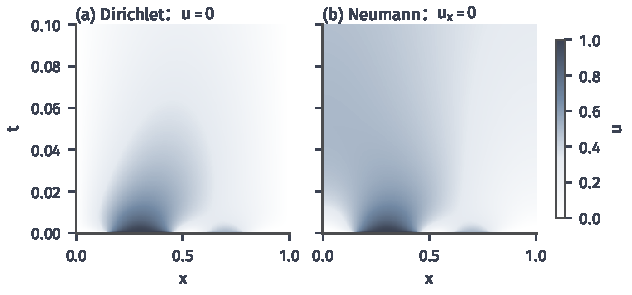
\includegraphics[width=107mm]{figures/03-optimization-evolution-and-signals/02-processes-and-trajectory-evolution/matplotlib/pde-heat-heatmap/figure.pdf}
  \caption{热方程$u_t=u_{xx}$的时空温度图，颜色越深温度越高。初值在$[0.15,0.45]$上为$1$、在$[0.6,0.8]$上为$0.5$，其余为零（边缘做了宽约$0.004$的光滑过渡）。(a)~两端Dirichlet条件$u=0$：温度整体衰减到零。(b)~两端Neumann条件$u_x=0$：温度趋于初值的均值$0.4$。由$400$项正弦与余弦级数计算。}
  \label{fig:pde-heat-heatmap}
\end{figure}

\subsection{弱演化与解算子}
\label{sec:pde-heat-semigroup}

模式展开依赖区间上显式的特征函数。在一般区域上，我们需要不依赖显式公式的框架：一种弱的解释，用能量估计得到唯一性与连续依赖；再把解看成作用在初值上的线性算子族。

\paragraph{弱形式中的时间与空间}
设$\Omega\subset\mathbb R^d$为有界开集，考虑$u_t=\Delta u+f$，边界为零，初值$u_0$。对固定的$t$，用$v\in H_0^1(\Omega)$检验并在空间上分部积分，得到
\begin{equation}
  \frac{\mathrm d}{\mathrm dt}\langle u(t),v\rangle+a\bigl(u(t),v\bigr)=\langle f(t),v\rangle\qquad\text{对所有}v\in H_0^1(\Omega),
  \label{eq:pde-heat-weak}
\end{equation}
其中$a(u,v)=\int_\Omega\nabla u\cdot\nabla v$与上一节相同。要让这个式子有意义，需要分别规定空间与时间上的正则性。在空间上，每个时刻的$u(t)$属于$H_0^1(\Omega)$，即零边界条件与一个弱导数；在时间上，$u$对$t$平方可积地取值于$H_0^1(\Omega)$，而$u_t$只要求取值于$H^{-1}(\Omega)$，这正好与$a(u(t),\cdot)$同属一个空间。初值$u_0$只需属于$L^2(\Omega)$。可以证明满足这些条件的$u$作为$[0,T]\to L^2(\Omega)$的映射是连续的，所以“$u(0)=u_0$”有意义。取值于函数空间的函数的积分（Bochner积分）这里不展开；下面凡需严格论证之处，都落在有限维的Galerkin逼近或区间上的模式展开中完成。

\paragraph{能量估计：唯一性与连续依赖}
在式~\eqref{eq:pde-heat-weak}中取$v=u(t)$。对上述函数类，可以证明$\langle u_t,u\rangle=\tfrac12\tfrac{\mathrm d}{\mathrm dt}\|u\|^2$，于是
\begin{equation}
  \frac12\frac{\mathrm d}{\mathrm dt}\|u(t)\|^2+\|\nabla u(t)\|^2=\langle f(t),u(t)\rangle .
  \label{eq:pde-heat-energy}
\end{equation}
无源时积分得
\[
  \frac12\|u(T)\|^2+\int_0^T\|\nabla u(t)\|^2\,\mathrm dt=\frac12\|u_0\|^2 .
\]
这个等式有两层含义。第一，$\|u(t)\|$不增：两个弱解之差是初值为零的弱解，它的范数恒为零，所以弱解唯一。第二，即使$u_0$只是平方可积、梯度可能处处不存在，梯度的平方在时间上的积分也被$\tfrac12\|u_0\|^2$控制，这是磨光效应的定量形式。有源时，用$|\langle f,u\rangle|\leq\|f\|_{H^{-1}}\|\nabla u\|\leq\tfrac12\|f\|_{H^{-1}}^2+\tfrac12\|\nabla u\|^2$吸收右端，得
\begin{equation}
  \|u(T)\|^2+\int_0^T\|\nabla u\|^2\,\mathrm dt\leq\|u_0\|^2+\int_0^T\|f(t)\|_{H^{-1}}^2\,\mathrm dt .
  \label{eq:pde-heat-energy-source}
\end{equation}
用于两组数据之差，就是初值与源项的连续依赖。

\paragraph{Galerkin逼近构造解}
唯一性与连续依赖来自能量估计，存在性则可以用有限维问题逼近得到。证明思路分三步。

第一步，选$H_0^1(\Omega)$中线性无关的$w_1,w_2,\ldots$，其有限线性组合在$H_0^1(\Omega)$中稠密，例如Dirichlet问题的特征函数。在$V_m=\operatorname{span}\{w_1,\ldots,w_m\}$中找$u_m(t)=\sum_{j=1}^mc_j(t)w_j$，只要求式~\eqref{eq:pde-heat-weak}对$v=w_1,\ldots,w_m$成立。记$\bm M_{i,j}=\langle w_j,w_i\rangle$、$\bm K_{i,j}=a(w_j,w_i)$、$\bm F_i(t)=\langle f(t),w_i\rangle$，条件化为
\[
  \bm M\bm c'(t)+\bm K\bm c(t)=\bm F(t),\qquad\bm c(0)\ \text{由}\ u_0\ \text{在}\ V_m\ \text{上的投影给出}.
\]
$\bm M$是Gram矩阵，对称正定，所以这是常系数线性常微分方程组，由第~\ref{chap:ordinary-differential-equations}章的线性理论在$[0,T]$上有唯一解。

第二步，在有限维中，能量估计~\eqref{eq:pde-heat-energy-source}可以严格推出：$\tfrac12\tfrac{\mathrm d}{\mathrm dt}\bm c^{\top}\bm M\bm c=\bm c^{\top}\bm M\bm c'$只是有限维求导。估计的右端与$m$无关，所以$(u_m)$在相应的函数空间中一致有界。第三步，Hilbert空间中的有界序列有弱收敛子列（这一结论在第~\ref{sec:pde-lax-milgram}小节引用过的卷二同一章中建立）；方程对$u_m$是线性的，对固定的检验函数可以在弱极限下取极限，极限就是弱解。这一构造与第~\ref{sec:pde-fem}小节的有限元方法同源：有限元正是取一组具体的$w_j$，并在有限的$m$处停下来计算。

\paragraph{解算子与半群性质}
固定$f=0$，把初值映到时刻$t$的解，得到映射$S(t):u_0\mapsto u(t)$。由唯一性与线性，$S(t)$是$L^2(\Omega)$上的线性算子；由能量估计，$\|S(t)u_0\|\leq\|u_0\|$。$S(0)$是恒等映射。从$u_0$出发走$t+s$的时间，与先走$s$到达$S(s)u_0$、再以它为初值走$t$，得到同一个解，因为二者在后一段时间满足同一个问题而解唯一，即$S(t+s)=S(t)S(s)$。最后$S(t)u_0\to u_0$，这是初值在$L^2$意义下取到。

上一章的线性系统$\dot{\bm x}=\bm A\bm x$有完全相同的结构：$e^{t\bm A}$满足$e^{0\bm A}=\bm I$与$e^{(t+s)\bm A}=e^{t\bm A}e^{s\bm A}$。热方程的解算子是这一结构在无限维中的对应物，在区间上它把每个$e_k$乘以$e^{-k^2\pi^2t}$，是一个“对角”的指数。

\begin{definition}[强连续半群]
\label{def:pde-c0-semigroup}
设$X$为Banach空间，$\{S(t)\}_{t\geq0}$是$X$上的有界线性算子族。若$S(0)=I$，$S(t+s)=S(t)S(s)$对所有$t,s\geq0$成立，并且对每个$x\in X$，$\lim_{t\to0^+}\|S(t)x-x\|=0$，则称它是\term{强连续半群}（strongly continuous semigroup）。若还有$\|S(t)\|\leq1$，称为压缩半群。
\end{definition}

“半群”指只有$t\geq0$：一般不能把时间倒过来，第~\ref{sec:pde-heat-long-time}小节会看到反向的热方程在何种程度上失效。“强连续”只要求对每个固定的$x$连续，不要求$\|S(t)-I\|\to0$；后者对热方程不成立，因为$\|S(t)e_k-e_k\|=1-e^{-k^2\pi^2t}$在$k\to\infty$时趋于$1$，无论$t$多小。

\paragraph{生成元与定义域}
矩阵指数由$\bm A$生成：$\bm A=\lim_{t\to0}(e^{t\bm A}-\bm I)/t$。对半群做同样的事。

\begin{definition}[生成元]
\label{def:pde-generator}
设$\{S(t)\}$为Banach空间$X$上的强连续半群。令$D(A)$为使极限$\lim_{t\to0^+}(S(t)x-x)/t$在$X$中存在的$x$全体，对$x\in D(A)$令$Ax$为该极限。称$A$为半群的\term{生成元}（generator），$D(A)$为它的定义域。
\end{definition}

区间上的热半群可以把生成元完全算出来。

\begin{theorem}[区间上热半群的生成元]
\label{thm:pde-heat-generator}
在$X=L^2(0,1)$上，设$S(t)$为式~\eqref{eq:pde-heat-series}给出的半群，$\lambda_k=k^2\pi^2$。则$u=\sum_kc_ke_k$属于$D(A)$当且仅当$\sum_k\lambda_k^2c_k^2<\infty$，此时$Au=-\sum_k\lambda_kc_ke_k$。若$u\in H^2(0,1)\cap H_0^1(0,1)$，则$u\in D(A)$且$Au=u''$。
\end{theorem}

\begin{proof}
设$\sum\lambda_k^2c_k^2<\infty$，令$y=-\sum\lambda_kc_ke_k$。则
\[
  \Bigl\|\frac{S(t)u-u}{t}-y\Bigr\|^2=\sum_k\Bigl(\frac{e^{-\lambda_kt}-1}{t}+\lambda_k\Bigr)^2c_k^2 .
\]
由$0\leq1-e^{-\lambda t}\leq\lambda t$，括号中的量属于$[0,\lambda_k]$，每一项不超过$\lambda_k^2c_k^2$，且对每个$k$在$t\to0^+$时趋于零；由控制收敛定理，和趋于零。反过来，若极限$y$存在，取第$k$个系数，$\langle y,e_k\rangle=\lim_{t\to0^+}\frac{e^{-\lambda_kt}-1}{t}c_k=-\lambda_kc_k$，由Parseval等式$\sum\lambda_k^2c_k^2=\|y\|^2<\infty$。

若$u\in H^2\cap H_0^1$，$u$与$e_k$在两端都为零，分部积分两次得$\langle u'',e_k\rangle=\langle u,e_k''\rangle=-\lambda_kc_k$，所以$\sum\lambda_k^2c_k^2=\|u''\|^2<\infty$，且$Au=\sum\langle u'',e_k\rangle e_k=u''$。
\end{proof}

这个计算显示了与矩阵情形的根本差别。$\|Ae_k\|=k^2\pi^2$无界，生成元不是有界算子，只在足够光滑、满足边界条件的函数上有定义；$e^{tA}$不能用幂级数$\sum t^nA^n/n!$定义，只能通过半群本身来理解。边界条件藏在定义域里：Neumann条件给出同一个微分表达式$u''$，但定义域不同，生成的半群也不同。

\paragraph{含源项：Duhamel公式与温和解}
有源项时，回想上一章的常数变易公式：$\dot{\bm x}=\bm A\bm x+\bm f(t)$的解是$\bm x(t)=e^{t\bm A}\bm x_0+\int_0^te^{(t-s)\bm A}\bm f(s)\,\mathrm ds$。区间上逐个模式做同样的计算：第$k$个系数满足标量方程$c_k'=-\lambda_kc_k+f_k(t)$，$f_k=\langle f,e_k\rangle$，所以
\[
  c_k(t)=e^{-\lambda_kt}c_k(0)+\int_0^te^{-\lambda_k(t-s)}f_k(s)\,\mathrm ds .
\]
把所有模式组装起来，就是
\begin{equation}
  u(t)=S(t)u_0+\int_0^tS(t-s)f(s)\,\mathrm ds ,
  \label{eq:pde-duhamel}
\end{equation}
称为\term{Duhamel公式}（Duhamel's formula）。右端可以这样读：时刻$s$注入的热量$f(s)\,\mathrm ds$此后自由扩散了$t-s$的时间，再与初值的扩散叠加。

设$f:[0,T]\to L^2(\Omega)$连续。半群一致有界且强连续，所以被积函数$s\mapsto S(t-s)f(s)$连续，式~\eqref{eq:pde-duhamel}可以作为取值于$L^2$的连续函数的Riemann积分理解。我们把由式~\eqref{eq:pde-duhamel}定义的$u$称为温和解。它不要求$u$可微，只要求半群存在，因而适用于数据较粗糙的情形；数据足够好时，可以证明它与弱解、经典解一致。

\begin{example}[恒定热源下趋于稳态]
\label{ex:pde-heat-steady-source}
在$(0,1)$上取$u_0=0$、恒定热源$f=1$、两端为零。$f$的系数为$f_k=\langle1,e_k\rangle$，由Duhamel公式$c_k(t)=f_k(1-e^{-\lambda_kt})/\lambda_k$。$t\to\infty$时$c_k(t)\to f_k/\lambda_k$，这正是稳态问题$-u''=1$的解$x(1-x)/2$的系数，因为$-u''=f$在模式坐标中就是$\lambda_kc_k=f_k$。每个模式以自己的速率$\lambda_k$接近稳态，最慢的是$k=1$。
\end{example}

\paragraph{一般区域上的生成元（补充）}
在一般有界区域上没有显式的特征函数，生成元要直接构造。令$D(A)$由满足下述条件的$u\in H_0^1(\Omega)$组成：存在$g\in L^2(\Omega)$，使$a(u,v)=-\langle g,v\rangle$对所有$v\in H_0^1(\Omega)$成立；对这样的$u$令$Au=g$，它是弱意义下的$\Delta u$。这个算子有两条性质。其一，$\langle Au,u\rangle=-\|\nabla u\|^2\leq0$，称为耗散的。其二，对每个$\lambda>0$与$f\in L^2(\Omega)$，方程$\lambda u-Au=f$可解，因为它的弱形式$\lambda\langle u,v\rangle+a(u,v)=\langle f,v\rangle$的双线性型在$H_0^1$上强制，可以用Lax--Milgram定理。泛函分析中的Lumer--Phillips定理说，稠密定义、耗散且$\lambda I-A$满射的算子恰好生成压缩半群；这里不加证明地引用它。于是热半群在一般区域上同样存在，前面的能量估计、半群性质和Duhamel公式都照样成立。

\subsection{能量、正性与长期极限}
\label{sec:pde-heat-long-time}

\paragraph{能量耗散、总热量守恒与边界泄漏}
本小节设解足够光滑，可以在空间上分部积分。考察两个量：能量$E(t)=\tfrac12\|u(t)\|^2$与总热量$Q(t)=\int_\Omega u(\bm x,t)\,\mathrm d\bm x$。无源时，
\[
  \begin{aligned}
    E'(t)&=\int_\Omega u\Delta u\,\mathrm d\bm x=-\|\nabla u\|^2+\int_{\partial\Omega}u\,\partial_{\bm n}u\,\mathrm dS,\\
    Q'(t)&=\int_\Omega\Delta u\,\mathrm d\bm x=\int_{\partial\Omega}\partial_{\bm n}u\,\mathrm dS .
  \end{aligned}
\]
零Dirichlet与零Neumann边界都使$E'$的边界项为零，所以$E'=-\|\nabla u\|^2\leq0$，能量耗散。总热量则不同：零Neumann边界下$Q'=0$，热量守恒；零Dirichlet边界下$Q'$等于穿过边界的净通量，正温度场在边界附近向零下降，$\partial_{\bm n}u\leq0$，热量从边界泄漏。

所以“能量耗散”“总量守恒”“边界泄漏”是三个不同的性质，不能互相推出。绝热的棒保持总热量，能量仍在减少：由Cauchy--Schwarz不等式$Q^2\leq|\Omega|\,\|u\|^2$，在总热量固定时，均匀分布的温度能量最小，扩散让温度趋于均匀，能量随之下降到这个最小值。图~\ref{fig:pde-heat-energy-max}(a)在两端为零的情形下比较了能量与总热量：二者都衰减，但速率不同。

\paragraph{弱最大值原理}
热量从热处流向冷处，所以内部不可能凭空出现比初始和边界更热的点。下面的定理把这一直觉变成证明，这类结论统称\term{最大值原理}（maximum principle）。记$\Omega_T=\Omega\times(0,T]$，称$\Gamma_T=(\overline\Omega\times\{0\})\cup(\partial\Omega\times[0,T])$为抛物边界，即底面与侧面，不含顶面。

\begin{theorem}[热方程的弱最大值原理]
\label{thm:pde-max-principle}
设$\Omega$为有界开集，$\kappa>0$，$u$在$\Omega_T$上关于$\bm x$二次、关于$t$一次连续可微，并在$\overline\Omega\times[0,T]$上连续。若在$\Omega_T$中$u_t-\kappa\Delta u\leq0$，则
\[
  \max_{\overline\Omega\times[0,T]}u=\max_{\Gamma_T}u .
\]
\end{theorem}

\begin{proof}
任取$\varepsilon>0$，令$v=u-\varepsilon t$，则在$\Omega_T$中$v_t-\kappa\Delta v=u_t-\kappa\Delta u-\varepsilon<0$。$v$在紧集$\overline\Omega\times[0,T]$上连续，在某点$(\bm x_0,t_0)$取到最大值。假设该点在$\Omega_T$中，即$\bm x_0\in\Omega$、$0<t_0\leq T$。固定$t_0$，$\bm x_0$是$v(\cdot,t_0)$的内部最大点，Hessian半负定，$\Delta v\leq0$。固定$\bm x_0$，若$t_0<T$则$v_t=0$；若$t_0=T$，$v(\bm x_0,t)\leq v(\bm x_0,T)$对$t<T$成立，左导数$v_t\geq0$。两种情形都有$v_t-\kappa\Delta v\geq0$，矛盾。所以最大值在$\Gamma_T$上取到，
\[
  \max u\leq\max v+\varepsilon T=\max_{\Gamma_T}v+\varepsilon T\leq\max_{\Gamma_T}u+\varepsilon T .
\]
令$\varepsilon\to0$即得。
\end{proof}

对$-u$使用定理，最小值也在抛物边界上取到。由此得到几个直接的推论。\term{比较原理}（comparison principle）：若$u_t-\kappa\Delta u\leq w_t-\kappa\Delta w$且在$\Gamma_T$上$u\leq w$，则处处$u\leq w$，只需对$u-w$使用定理。正性：无源时，初值与边界值非负，则解处处非负。稳定性与唯一性：两个经典解之差满足$\max|u_1-u_2|\leq\max_{\Gamma_T}|u_1-u_2|$，数据相同则解相同。图~\ref{fig:pde-heat-energy-max}(b)画出了初值$\sin(\pi x)+\sin(5\pi x)$的最大值$M(t)$与最小值$m(t)$：前者单调不增，后者从$-0.198$单调回升到零，从未越出初值的范围。定理~\ref{thm:pde-max-principle}在上述的弱形式中也有相应版本，这里只讨论经典解。

\begin{figure}[!htb]
  \centering
  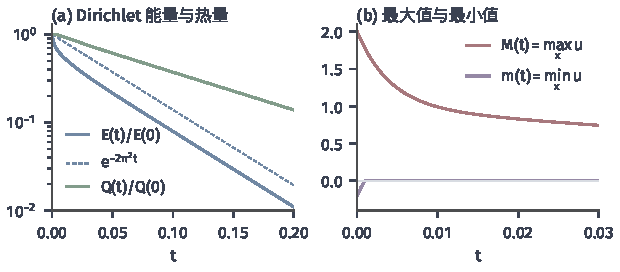
\includegraphics[width=105mm]{figures/03-optimization-evolution-and-signals/02-processes-and-trajectory-evolution/matplotlib/pde-heat-energy-max/figure.pdf}
  \caption{两端为零的热方程$u_t=u_{xx}$中的能量、热量与极值。(a)~初值与图~\ref{fig:pde-heat-heatmap}相同，能量$E=\tfrac12\|u\|^2$与总热量$Q=\int u$都相对初值归一化，纵轴为对数刻度；虚线$e^{-2\pi^2t}$是由Poincaré不等式得到的能量上界。(b)~初值$\sin(\pi x)+\sin(5\pi x)$的空间最大值$M(t)$与最小值$m(t)$，二者都不越出初值和边界值的范围。}
  \label{fig:pde-heat-energy-max}
\end{figure}

\paragraph{长期行为：衰减、均值与稳态}
在零Dirichlet边界下，由Poincaré不等式$\|\nabla u\|^2\geq\|u\|^2/C_P^2$，能量满足$E'\leq-2E/C_P^2$，于是$\frac{\mathrm d}{\mathrm dt}\bigl(e^{2t/C_P^2}E\bigr)\leq0$，
\[
  \|u(t)\|\leq e^{-t/C_P^2}\|u_0\| .
\]
在$(0,1)$上$C_P=1/\pi$，速率$\pi^2$正是最低模式的衰减率，与定理~\ref{thm:pde-heat-series}一致；图~\ref{fig:pde-heat-energy-max}(a)的虚线就是这个界。

在零Neumann边界下，总热量守恒，均值$\bar u=Q/|\Omega|$不随时间变化。$w=u-\bar u$满足同一方程、同一边界条件，且均值为零；设$\Omega$为有界连通Lipschitz区域，由零均值的Poincaré不等式，同样的论证给出$\|u(t)-\bar u\|\leq e^{-t/C^2}\|u_0-\bar u\|$。解趋于初值的均值，不趋于零，这就是图~\ref{fig:pde-heat-heatmap}(b)中的现象。

有不随时间变化的源$f\in L^2(\Omega)$时，零Dirichlet边界下令$u_\infty$为Poisson问题$-\Delta u_\infty=f$的弱解。$w=u-u_\infty$满足无源的热方程，初值为$u_0-u_\infty$，所以$\|u(t)-u_\infty\|\leq e^{-t/C_P^2}\|u_0-u_\infty\|$：有源时解趋于稳态，而不是趋于零，例~\ref{ex:pde-heat-steady-source}是它的具体情形。零Neumann边界下，若$\int_\Omega f\neq0$，则$Q'=\int_\Omega f$，总热量线性增长，没有稳态；这正是第~\ref{sec:pde-other-boundary}小节的相容条件在时间中的表现，图~\ref{fig:pde-neumann}(b)画出了这种情形。

\paragraph{反向热方程不适定}
磨光效应的另一面是信息的丢失。设已知时刻$T$的温度，反推初值。在区间上，$c_k(0)=e^{k^2\pi^2T}c_k(T)$。若时刻$T$的观测有一个大小为$\delta$的高频误差$\delta e_k$，反推出的初值误差就是$\delta e^{k^2\pi^2T}e_k$。取$T=0.1$、$k=5$，放大倍数$e^{2.5\pi^2}\approx5\times10^{10}$；$k$越大放大越厉害，没有上界。所以反向问题在$L^2$中不满足连续依赖，按第~\ref{sec:pde-boundary-solution-meaning}小节的定义是不适定的。正向演化把高频成分压到几乎为零，反向演化就必须把几乎为零的成分重新放大。

本节始终把$u$当作确定性的温度场。热方程还有一个概率的读法：它也描述随机游走的粒子在空间中的密度怎样随时间扩散。这一联系需要随机过程的生成元，留到第~\ref{chap:continuous-time-stochastic-processes}章建立。
